\documentclass{article}
\usepackage[utf8]{inputenc}
\usepackage{graphicx}

\title{Physics 111 Lab 01: Position and Velocity}
\author{Noman Ahmad}
\date{Due Date: Feb 11, 2021}

\begin{document}

\maketitle

\section{Introduction}

\subsection{Background Information}
In this lab, we explored measuring and calculating position and velocity. Anytime we perform any of the calculations regarding distance, position, displacement, speed, or velocity we must do so with respect to a reference frame. All of these different physical definitions will have different values depending on the reference frame. For example, someone sitting on an airplane will have 0 m/s speed with respect to the plane, but their speed will be much higher with respect to someone seeing the plane they are sitting in, fly by. For this lab, we use the xy-axis, also known as the cartesian coordinate plane as our reference frame. We measured and calculated speed, velocity, distance, and displacement using an online simulator in hopes to classify their differences in traditional one-dimensional physics. 

\subsection{Theory and Definitions}
\textbf{Distance} is a scalar quantity representing the total travel path for an object. Distance is always a positive value, and because of it's scalar property, it only has magnitude, not direction. \textbf{Displacement} on the other hand, is a vector quantity, representing both magnitude and direction along a path. It is a representation of how far an object has traveled with respect to its starting point. \\ \\ 
\textbf{Speed} is the total distance for an object with respect to a certain time interval. The average speed of an object is the distance the object traveled per the time it traveled. Speed, like distance is a scalar quantity and thus can't be negative. \textbf{Velocity} on the other hand represents the total displacement for an object with respect to a certain time level. Like displacement, velocity has both directional and magnitude properties, due to it being a vector. \\ \\ 
In many cases, speed and the magnitude of velocity are equal, however in no case can the magnitude of velocity be greater than speed. Speed can, however be greater than the magnitude of velocity. Similarly, distance can be equal to the magnitude of displacement, however the magnitude of displacement can never be greater than distance. In this lab, we hoped to find results consistent with this fact. 

\subsection{Relevant Formula's}
Displacement: \(\Delta x = x_2-x_1\) \\
Average Speed: \(\Delta s = \frac{x}{t}\) \\ 
Average Velocity: \(\Delta v = \frac{\Delta x} {\Delta t}\) \\ 
Position: \(x(t) = v_0t + x_0\)

\section{Results}
\subsection{Setup} 
In order to properly observe and measure the characteristics of speed, distance, velocity, and displacement in a one-dimensional setting we made use of a online simulator, which allowed us to retrieve real-time visualization of motion by displaying position per time and velocity per time plots in a zero acceleration manner. We then performed various operations using this online simulator. 
\subsection {Part One Results}
The first operation we did was use the online simulator to determine starting positions and determine the velocities for different time intervals on a plot, that would result in a given position plot, for a total of 5 different result plots. In order to do this, we would move the position slider until it reached the correct starting position, and then we would observe the required plot, and determine which time intervals require which velocities, and we would move the velocity slider appropriately. For example, if the object was staying in place in a designated time interval on the desired plot, we would move the velocity slider to 0m/s. After the plot would finish, we used the formulas to calculate the speed, displacement, distance, and velocity. The following is the observed data from the 5 different plots. In a few cases, such as the last two examples, we can see that the displacement and distance are different values as well as the speed and velocity, respectively. This reiterates the original point mentioned in the introduction, and you will also notice that the magnitude of the displacement in both cases (removing the signs), is still less than that of the distance, and that the magnitude of the velocity is also less than that of the speed, which stays consistent with what was established earlier. 
\begin{center}
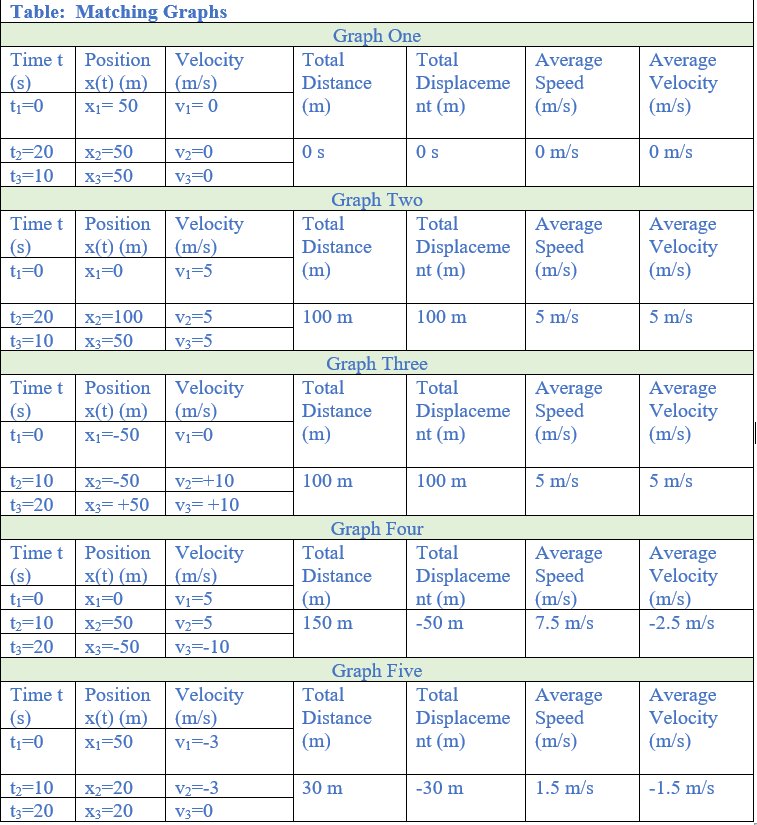
\includegraphics[scale=0.6]{data1.png}
\end{center}
\subsection {Part Two Results}
The second operation was working with position in a constant velocity setting. We chose a random velocity from 0 to 10 m/s, and we observed how long it would take for the position of the object to go from 0m to 100m in this setting. Afterwards, we broke the plot into 4 quarters of equal time length, and observed the slope of the position vs. time graph and we observed whether the slope would be the same as the velocity we chose. In this scenario, I chose my slope to be 8 m/s. Here are the results that I observed. 
\begin{center}
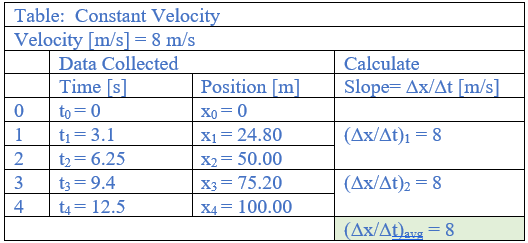
\includegraphics[scale=0.65]{data2.png}
\end{center}
\subsection{Part Three Results} 
For the final parts of our measurements, we needed to find the percent error between the observed positions from our plot/graph in the online simulator, and the position using the initial position and velocity using the formula, \(x(t) = v_0t + x_0\). I did this for a total of three times including the second, third, and fourth quarter positions of the plot resulting from the slope that I chose. For example, my second quarter position at \(t=6.25s\) was \(x_2=50.00m\) found by calculating the slope between \(t_2\) and \(t_0\). Here is a sample calculation that I performed using the formula: 
\begin{center} 
\(x(t) = v_0t+x_0\) \\ 
\(x(6.25) = \frac{8m}{s}6.25s + 0\) \\
\(x(6.25) = 8m(6.25)\) \\
\(x(6.5) = 50m\) \\
\end{center} 
In this scenario, both the results were the same, therefore the percent error was 0 percent. This can further be shown by using the percent error formula.
\begin{center}
\(\frac{|50.0m-50.0m|}{50.0m} x 100\% = 0\%\)
\end{center}
Similarly, I followed the same logic for the remaining two cases, and then found the percent error results to be exactly the same, here are the results. 
\begin{center}
    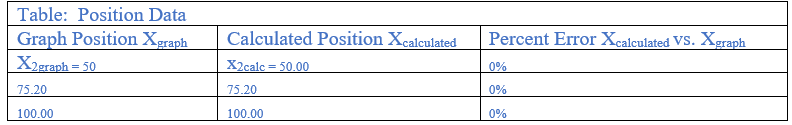
\includegraphics[scale=0.7]{data3.PNG}
\end{center}
\subsection{Conclusions} 
As expected there was no error between the formula's result of the position at a given time using the velocity, and the graphical representation. The derivations of the formula must have come after the graphical observation of such, and therefore the representations should be the exact same, which we observed is true and consistent. 
\section{Post-Lab Questions} 
\subsection{Problem 1} 
The figure shows a graph of the position of a moving object as a function of time. What is the velocity of the object at each of the following times? \\ \\
a) At \(t=1.0s\), finding the slope of the first line segment between t=0s and t=2s, we get 20m - 0m / 2s - 0s = 10m/s. Therefore the velocity at any point in the first two seconds in \textbf{10m/s}. \\ 
b) At \(t=2.5s\), similar to a, we find the slope of this current line segment between t=2s and t=3s, we get 40m-20m /3s-2s = 20m/1s = 20m/s. Therefore, the velocity at any point between t=2s and t=3s is \textbf{20m/s} \\ \\
c) At \(t=4.0s\), we would follow the same pattern as the first two by finding the slope of the line segment between t=3s and t=5s, in this case it is 0, therefore all points between t=3s and t=5s have a constant velocity of \textbf{0m/s}. \\ \\ 
d) At \(t=5.5s\), similar to above, the slope would be calculated between t=5s and t=6s. In this case, it would 0m-40m/6s-5s, which is -40m/s. This indicates a negative direction for the velocity. The velocity here is \textbf{-40m/s}.\\ \\ 
e) Average velocity from t=0s to t=4.0s, the formula for average velocity is displacement/time. Since the object started at x=0 at t=4, and is at x=40 at t=4, we would do the following, avg velocity = 40m-0m/4s-0s = 10m/s. Therefore the average velocity here is \textbf{10m/s}. \\ \\ 
f) Average velocity from t=0s to t=6.0s, similar to above we would do 0m-0m/6s-0s = 0m/s. Therefore the average velocity in this entire 6 seconds is \textbf{0m/s}. 
\begin{center} 
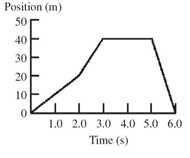
\includegraphics[scale=0.6]{postlab1.jpg}
\end{center}
\subsection{Problem 2} 
The graph in the figure shows the position of an object as a function of time. The letters H-L represent particular moments of time. 
\begin{center} 
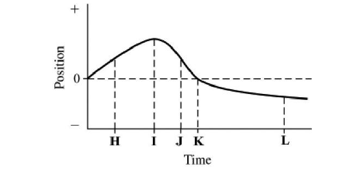
\includegraphics[scale=0.6]{postlab2.png}
\end{center}
a) \textit{At which moment in time is the speed of the object the greatest?} \\ 
We are already aware that on a position vs time graph, the velocity is represented as the slope of the given time intervals. In this case, \textbf{H}, because it has the greatest slope.\\ \\ 
b) \textit{At which moment in time is the speed of the object equal to zero?} \\
As described above, the only point with a velocity with magnitude 0 is I, therefore speed of the object is 0 m/s at point \textbf{I}. \\ \\ 
\subsection{Problem 3} 
If you run a complete loop around an outdoor track of length 400 m in 100s, find your \\ \\
a) \textit{Average Velocity} \\
Since you loop back around, the displacement is 0m, since you return back to your origin, therefore velocity is 0m/100s = \textbf{0m/s}. \\ \\ 
b) \textit{Average Speed} \\
Here we can use the formula avg speed = total distance / total time. In this case, the total distance is 800m, because it is 400m front and 400m back since it is a loop, therefore we can say average speed = 800m/100s = \textbf{8.0m/s}. \\
\subsection{Problem 4} 
A polar bear starts at the North Pole. It travels 1.0km south, then 1.0km east, and then returns to its starting point. This trip takes 0.75 hr.\\ \\
a) \textit{What was the bear's average speed?} \\ 
The formula for speed is total distance / total time. In this case, the polar bear walks 1 km south + 1 km east = 2km. He also has to return to his starting point so the total distance is 2km + 2km = 4km. Therefore, the total speed is 4km/0.75hr = \textbf{5.33km/hr}. \\ \\ 
b) \textit{What was the bear's average velocity?} \\
In this case, since the bear returned back to his original position, the average velocity in this case would be \textbf{0km/hr}.\\ 
\subsection{Problem 5} 
Two locomotives 70 kilometers apart are travelling on the same track towards each other , Engine A  moves at 22 kilometers per hour east  and engine B moves at 13 kilometers per hour west.  At the instant both trains begin moving, an annoying mutant fly begins flying from engine A towards engine B at 33 kilometers per hour . The instant it touches B, it turns around and flies back. It goes on  this way until the two locomotives collide and the mutant fly is finally squashed. So before its untimely demise determine the following: \\ \\
a. \textit{the total distance the fly flew}\\ 
    Position Equation for A: x(t) = 22t \\
    Position Equation for B: x(t) = -13t + 70 \\
    Position Equation for fly: x(t) = 33t \\
    A meets B: 22t = -13t + 70, 35t = 70, t = 70/35, t=2hr. \\
    Distance fly flew total: x(2) = 33(2) = \textbf{66km}. \\ \\
b. \textit{The time it took till it was eliminated.}\\
    Mentioned above, when A and B meet, that is \textbf{2hr} from the start. \\ \\ 
c. \textit{The average velocity of the fly} \\ 
    Time fly Meets B: 33t = -13t + 70, 46t=70, t= 70/46, t=1.53hrs. \\
    Distance Fly Travels to B: x(1.53) = 33(1.53) = 50.49km. \\
    Distance Fly Travels for Remaining Time (2-1.53): x(0.47) = -33(0.47) = -15.51km. (Note it turned around, hence negative). \\ 
    Total Displacement of Fly: 50.49km + -15.51km = 34.98km. \\ 
    Average Velocity of Fly: 34.98km/2hrs = \textbf{17.49km/hr}
\section{Discussion} 
The experiment was a success because we did not run into any inconsistencies when doing our measurements and calculations. We did not run into an instance where the magnitude of velocity or displacement was greater than speed or distance, which we know can not be true. We also did not run into any scenario where the results of the position equation gave us different results than the graphical representation of the same object. All of the results from the experiment stayed consistent with the theoretical concepts. These were exactly the results that we would expect, and we were able to successfully attain them without any error at all. 

\section{Sources}
1. Online Simulator: http://physics.bu.edu/~duffy/HTML5/1Dmotion\_graph\_matching.html 
\end{document}
